%\documentclass[slides]{beamer} %switch "slides" to "handout" for printing out
\documentclass[handout]{beamer}

%packages
%\usepackage{latexsym}
\usepackage{graphicx}
\usepackage{color}
\usepackage{amsmath}
\usepackage{dsfont}
\usepackage{placeins}
\usepackage{amssymb}
\usepackage{wasysym}
\usepackage{abstract}
\usepackage{hyperref}
\usepackage{etoolbox}
\usepackage{datetime}
\usepackage{xcolor}
\usepackage{alphalph}
\settimeformat{ampmtime}

%\usepackage{pstricks,pst-node,pst-tree}

%\usepackage{algpseudocode}
%\usepackage{amsthm}
%\usepackage{hyperref}
%\usepackage{mathrsfs}
%\usepackage{amsfonts}
%\usepackage{bbding}
%\usepackage{listings}
%\usepackage{appendix}
\usepackage[margin=1in]{geometry}
%\geometry{papersize={8.5in,11in},total={6.5in,9in}}
%\usepackage{cancel}
%\usepackage{algorithmic, algorithm}

\makeatletter
\def\maxwidth{ %
  \ifdim\Gin@nat@width>\linewidth
    \linewidth
  \else
    \Gin@nat@width
  \fi
}
\makeatother

\definecolor{fgcolor}{rgb}{0.345, 0.345, 0.345}
\newcommand{\hlnum}[1]{\textcolor[rgb]{0.686,0.059,0.569}{#1}}%
\newcommand{\hlstr}[1]{\textcolor[rgb]{0.192,0.494,0.8}{#1}}%
\newcommand{\hlcom}[1]{\textcolor[rgb]{0.678,0.584,0.686}{\textit{#1}}}%
\newcommand{\hlopt}[1]{\textcolor[rgb]{0,0,0}{#1}}%
\newcommand{\hlstd}[1]{\textcolor[rgb]{0.345,0.345,0.345}{#1}}%
\newcommand{\hlkwa}[1]{\textcolor[rgb]{0.161,0.373,0.58}{\textbf{#1}}}%
\newcommand{\hlkwb}[1]{\textcolor[rgb]{0.69,0.353,0.396}{#1}}%
\newcommand{\hlkwc}[1]{\textcolor[rgb]{0.333,0.667,0.333}{#1}}%
\newcommand{\hlkwd}[1]{\textcolor[rgb]{0.737,0.353,0.396}{\textbf{#1}}}%

\usepackage{framed}
\makeatletter
\newenvironment{kframe}{%
 \def\at@end@of@kframe{}%
 \ifinner\ifhmode%
  \def\at@end@of@kframe{\end{minipage}}%
  \begin{minipage}{\columnwidth}%
 \fi\fi%
 \def\FrameCommand##1{\hskip\@totalleftmargin \hskip-\fboxsep
 \colorbox{shadecolor}{##1}\hskip-\fboxsep
     % There is no \\@totalrightmargin, so:
     \hskip-\linewidth \hskip-\@totalleftmargin \hskip\columnwidth}%
 \MakeFramed {\advance\hsize-\width
   \@totalleftmargin\z@ \linewidth\hsize
   \@setminipage}}%
 {\par\unskip\endMakeFramed%
 \at@end@of@kframe}
\makeatother

\definecolor{shadecolor}{rgb}{.77, .77, .77}
\definecolor{messagecolor}{rgb}{0, 0, 0}
\definecolor{warningcolor}{rgb}{1, 0, 1}
\definecolor{errorcolor}{rgb}{1, 0, 0}
\newenvironment{knitrout}{}{} % an empty environment to be redefined in TeX

\usepackage{alltt}
\usepackage[T1]{fontenc}

\newcommand{\qu}[1]{``#1''}
\newcounter{probnum}
\setcounter{probnum}{1}

%create definition to allow local margin changes
\def\changemargin#1#2{\list{}{\rightmargin#2\leftmargin#1}\item[]}
\let\endchangemargin=\endlist 

%allow equations to span multiple pages
\allowdisplaybreaks

%define colors and color typesetting conveniences
\definecolor{gray}{rgb}{0.5,0.5,0.5}
\definecolor{black}{rgb}{0,0,0}
\definecolor{white}{rgb}{1,1,1}
\definecolor{blue}{rgb}{0.5,0.5,1}
\newcommand{\inblue}[1]{\color{blue}#1 \color{black}}
\definecolor{green}{rgb}{0.133,0.545,0.133}
\newcommand{\ingreen}[1]{\color{green}#1 \color{black}}
\definecolor{yellow}{rgb}{1,1,0}
\newcommand{\inyellow}[1]{\color{yellow}#1 \color{black}}
\definecolor{orange}{rgb}{0.9,0.649,0}
\newcommand{\inorange}[1]{\color{orange}#1 \color{black}}
\definecolor{red}{rgb}{1,0.133,0.133}
\newcommand{\inred}[1]{\color{red}#1 \color{black}}
\definecolor{purple}{rgb}{0.58,0,0.827}
\newcommand{\inpurple}[1]{\color{purple}#1 \color{black}}
\definecolor{backgcode}{rgb}{0.97,0.97,0.8}
\definecolor{Brown}{cmyk}{0,0.81,1,0.60}
\definecolor{OliveGreen}{cmyk}{0.64,0,0.95,0.40}
\definecolor{CadetBlue}{cmyk}{0.62,0.57,0.23,0}

%define new math operators
\DeclareMathOperator*{\argmax}{arg\,max~}
\DeclareMathOperator*{\argmin}{arg\,min~}
\DeclareMathOperator*{\argsup}{arg\,sup~}
\DeclareMathOperator*{\arginf}{arg\,inf~}
\DeclareMathOperator*{\convolution}{\text{\Huge{$\ast$}}}
\newcommand{\infconv}[2]{\convolution^\infty_{#1 = 1} #2}
%true functions

%%%% GENERAL SHORTCUTS

%shortcuts for pure typesetting conveniences
\newcommand{\bv}[1]{\boldsymbol{#1}}

%shortcuts for compound constants
\newcommand{\BetaDistrConst}{\dfrac{\Gamma(\alpha + \beta)}{\Gamma(\alpha)\Gamma(\beta)}}
\newcommand{\NormDistrConst}{\dfrac{1}{\sqrt{2\pi\sigma^2}}}

%shortcuts for conventional symbols
\newcommand{\tsq}{\tau^2}
\newcommand{\tsqh}{\hat{\tau}^2}
\newcommand{\sigsq}{\sigma^2}
\newcommand{\sigsqsq}{\parens{\sigma^2}^2}
\newcommand{\sigsqovern}{\dfrac{\sigsq}{n}}
\newcommand{\tausq}{\tau^2}
\newcommand{\tausqalpha}{\tau^2_\alpha}
\newcommand{\tausqbeta}{\tau^2_\beta}
\newcommand{\tausqsigma}{\tau^2_\sigma}
\newcommand{\betasq}{\beta^2}
\newcommand{\sigsqvec}{\bv{\sigma}^2}
\newcommand{\sigsqhat}{\hat{\sigma}^2}
\newcommand{\sigsqhatmlebayes}{\sigsqhat_{\text{Bayes, MLE}}}
\newcommand{\sigsqhatmle}[1]{\sigsqhat_{#1, \text{MLE}}}
\newcommand{\bSigma}{\bv{\Sigma}}
\newcommand{\bSigmainv}{\bSigma^{-1}}
\newcommand{\thetavec}{\bv{\theta}}
\newcommand{\thetahat}{\hat{\theta}}
\newcommand{\thetahatmle}{\hat{\theta}_{\mathrm{MLE}}}
\newcommand{\thetavechatmle}{\hat{\thetavec}_{\mathrm{MLE}}}
\newcommand{\muhat}{\hat{\mu}}
\newcommand{\musq}{\mu^2}
\newcommand{\muvec}{\bv{\mu}}
\newcommand{\muhatmle}{\muhat_{\text{MLE}}}
\newcommand{\lambdahat}{\hat{\lambda}}
\newcommand{\lambdahatmle}{\lambdahat_{\text{MLE}}}
\newcommand{\etavec}{\bv{\eta}}
\newcommand{\alphavec}{\bv{\alpha}}
\newcommand{\minimaxdec}{\delta^*_{\mathrm{mm}}}
\newcommand{\ybar}{\bar{y}}
\newcommand{\xbar}{\bar{x}}
\newcommand{\Xbar}{\bar{X}}
\newcommand{\phat}{\hat{p}}
\newcommand{\Phat}{\hat{P}}
\newcommand{\Zbar}{\bar{Z}}
\newcommand{\iid}{~{\buildrel iid \over \sim}~}
\newcommand{\inddist}{~{\buildrel ind \over \sim}~}
\newcommand{\approxdist}{~{\buildrel approx \over \sim}~}
\newcommand{\equalsindist}{~{\buildrel d \over =}~}
\newcommand{\loglik}[1]{\ell\parens{#1}}
\newcommand{\thetahatkminone}{\thetahat^{(k-1)}}
\newcommand{\thetahatkplusone}{\thetahat^{(k+1)}}
\newcommand{\thetahatk}{\thetahat^{(k)}}
\newcommand{\half}{\frac{1}{2}}
\newcommand{\third}{\frac{1}{3}}
\newcommand{\twothirds}{\frac{2}{3}}
\newcommand{\fourth}{\frac{1}{4}}
\newcommand{\fifth}{\frac{1}{5}}
\newcommand{\sixth}{\frac{1}{6}}

%shortcuts for vector and matrix notation
\newcommand{\A}{\bv{A}}
\newcommand{\At}{\A^T}
\newcommand{\Ainv}{\inverse{\A}}
\newcommand{\B}{\bv{B}}
\newcommand{\K}{\bv{K}}
\newcommand{\Kt}{\K^T}
\newcommand{\Kinv}{\inverse{K}}
\newcommand{\Kinvt}{(\Kinv)^T}
\newcommand{\M}{\bv{M}}
\newcommand{\Bt}{\B^T}
\newcommand{\Q}{\bv{Q}}
\newcommand{\Qt}{\Q^T}
\newcommand{\R}{\bv{R}}
\newcommand{\Rt}{\R^T}
\newcommand{\Z}{\bv{Z}}
\newcommand{\X}{\bv{X}}
\newcommand{\Xsub}{\X_{\text{(sub)}}}
\newcommand{\Xsubadj}{\X_{\text{(sub,adj)}}}
\newcommand{\I}{\bv{I}}
\newcommand{\Y}{\bv{Y}}
\newcommand{\sigsqI}{\sigsq\I}
\renewcommand{\P}{\bv{P}}
\newcommand{\Psub}{\P_{\text{(sub)}}}
\newcommand{\Pt}{\P^T}
\newcommand{\Pii}{P_{ii}}
\newcommand{\Pij}{P_{ij}}
\newcommand{\IminP}{(\I-\P)}
\newcommand{\Xt}{\bv{X}^T}
\newcommand{\XtX}{\Xt\X}
\newcommand{\XtXinv}{\parens{\Xt\X}^{-1}}
\newcommand{\XtXinvXt}{\XtXinv\Xt}
\newcommand{\XXtXinvXt}{\X\XtXinvXt}
\newcommand{\x}{\bv{x}}
\newcommand{\onevec}{\bv{1}}
\newcommand{\oneton}{1, \ldots, n}
\newcommand{\yoneton}{y_1, \ldots, y_n}
\newcommand{\yonetonorder}{y_{(1)}, \ldots, y_{(n)}}
\newcommand{\Yoneton}{Y_1, \ldots, Y_n}
\newcommand{\iinoneton}{i \in \braces{\oneton}}
\newcommand{\onetom}{1, \ldots, m}
\newcommand{\jinonetom}{j \in \braces{\onetom}}
\newcommand{\xoneton}{x_1, \ldots, x_n}
\newcommand{\Xoneton}{X_1, \ldots, X_n}
\newcommand{\xt}{\x^T}
\newcommand{\y}{\bv{y}}
\newcommand{\yt}{\y^T}
\renewcommand{\c}{\bv{c}}
\newcommand{\ct}{\c^T}
\newcommand{\tstar}{\bv{t}^*}
\renewcommand{\u}{\bv{u}}
\renewcommand{\v}{\bv{v}}
\renewcommand{\a}{\bv{a}}
\newcommand{\s}{\bv{s}}
\newcommand{\yadj}{\y_{\text{(adj)}}}
\newcommand{\xjadj}{\x_{j\text{(adj)}}}
\newcommand{\xjadjM}{\x_{j \perp M}}
\newcommand{\yhat}{\hat{\y}}
\newcommand{\yhatsub}{\yhat_{\text{(sub)}}}
\newcommand{\yhatstar}{\yhat^*}
\newcommand{\yhatstarnew}{\yhatstar_{\text{new}}}
\newcommand{\z}{\bv{z}}
\newcommand{\zt}{\z^T}
\newcommand{\bb}{\bv{b}}
\newcommand{\bbt}{\bb^T}
\newcommand{\bbeta}{\bv{\beta}}
\newcommand{\betahat}{\hat{\beta}}
\newcommand{\beps}{\bv{\epsilon}}
\newcommand{\bepst}{\beps^T}
\newcommand{\e}{\bv{e}}
\newcommand{\Mofy}{\M(\y)}
\newcommand{\KofAlpha}{K(\alpha)}
\newcommand{\ellset}{\mathcal{L}}
\newcommand{\oneminalph}{1-\alpha}
\newcommand{\SSE}{\text{SSE}}
\newcommand{\SSEsub}{\text{SSE}_{\text{(sub)}}}
\newcommand{\MSE}{\text{MSE}}
\newcommand{\RMSE}{\text{RMSE}}
\newcommand{\SSR}{\text{SSR}}
\newcommand{\SST}{\text{SST}}
\newcommand{\JSest}{\delta_{\text{JS}}(\x)}
\newcommand{\Bayesest}{\delta_{\text{Bayes}}(\x)}
\newcommand{\EmpBayesest}{\delta_{\text{EmpBayes}}(\x)}
\newcommand{\BLUPest}{\delta_{\text{BLUP}}}
\newcommand{\MLEest}[1]{\hat{#1}_{\text{MLE}}}

%shortcuts for Linear Algebra stuff (i.e. vectors and matrices)
\newcommand{\twovec}[2]{\bracks{\begin{array}{c} #1 \\ #2 \end{array}}}
\newcommand{\threevec}[3]{\bracks{\begin{array}{c} #1 \\ #2 \\ #3 \end{array}}}
\newcommand{\fivevec}[5]{\bracks{\begin{array}{c} #1 \\ #2 \\ #3 \\ #4 \\ #5 \end{array}}}
\newcommand{\twobytwomat}[4]{\bracks{\begin{array}{cc} #1 & #2 \\ #3 & #4 \end{array}}}
\newcommand{\threebytwomat}[6]{\bracks{\begin{array}{cc} #1 & #2 \\ #3 & #4 \\ #5 & #6 \end{array}}}

%shortcuts for conventional compound symbols
\newcommand{\thetainthetas}{\theta \in \Theta}
\newcommand{\reals}{\mathbb{R}}
\newcommand{\complexes}{\mathbb{C}}
\newcommand{\rationals}{\mathbb{Q}}
\newcommand{\integers}{\mathbb{Z}}
\newcommand{\naturals}{\mathbb{N}}
\newcommand{\forallninN}{~~\forall n \in \naturals}
\newcommand{\forallxinN}[1]{~~\forall #1 \in \reals}
\newcommand{\matrixdims}[2]{\in \reals^{\,#1 \times #2}}
\newcommand{\inRn}[1]{\in \reals^{\,#1}}
\newcommand{\mathimplies}{\quad\Rightarrow\quad}
\newcommand{\mathlogicequiv}{\quad\Leftrightarrow\quad}
\newcommand{\eqncomment}[1]{\quad \text{(#1)}}
\newcommand{\limitn}{\lim_{n \rightarrow \infty}}
\newcommand{\limitN}{\lim_{N \rightarrow \infty}}
\newcommand{\limitd}{\lim_{d \rightarrow \infty}}
\newcommand{\limitt}{\lim_{t \rightarrow \infty}}
\newcommand{\limitsupn}{\limsup_{n \rightarrow \infty}~}
\newcommand{\limitinfn}{\liminf_{n \rightarrow \infty}~}
\newcommand{\limitk}{\lim_{k \rightarrow \infty}}
\newcommand{\limsupn}{\limsup_{n \rightarrow \infty}}
\newcommand{\limsupk}{\limsup_{k \rightarrow \infty}}
\newcommand{\floor}[1]{\left\lfloor #1 \right\rfloor}
\newcommand{\ceil}[1]{\left\lceil #1 \right\rceil}

%shortcuts for environments
\newcommand{\beqn}{\vspace{-0.25cm}\begin{eqnarray*}}
\newcommand{\eeqn}{\end{eqnarray*}}
\newcommand{\bneqn}{\vspace{-0.25cm}\begin{eqnarray}}
\newcommand{\eneqn}{\end{eqnarray}}

%shortcuts for mini environments
\newcommand{\parens}[1]{\left(#1\right)}
\newcommand{\squared}[1]{\parens{#1}^2}
\newcommand{\tothepow}[2]{\parens{#1}^{#2}}
\newcommand{\prob}[1]{\mathbb{P}\parens{#1}}
\newcommand{\cprob}[2]{\prob{#1~|~#2}}
\newcommand{\littleo}[1]{o\parens{#1}}
\newcommand{\bigo}[1]{O\parens{#1}}
\newcommand{\Lp}[1]{\mathbb{L}^{#1}}
\renewcommand{\arcsin}[1]{\text{arcsin}\parens{#1}}
\newcommand{\prodonen}[2]{\bracks{\prod_{#1=1}^n #2}}
\newcommand{\mysum}[4]{\sum_{#1=#2}^{#3} #4}
\newcommand{\sumonen}[2]{\sum_{#1=1}^n #2}
\newcommand{\infsum}[2]{\sum_{#1=1}^\infty #2}
\newcommand{\infprod}[2]{\prod_{#1=1}^\infty #2}
\newcommand{\infunion}[2]{\bigcup_{#1=1}^\infty #2}
\newcommand{\infinter}[2]{\bigcap_{#1=1}^\infty #2}
\newcommand{\infintegral}[2]{\int^\infty_{-\infty} #2 ~\text{d}#1}
\newcommand{\supthetas}[1]{\sup_{\thetainthetas}\braces{#1}}
\newcommand{\bracks}[1]{\left[#1\right]}
\newcommand{\braces}[1]{\left\{#1\right\}}
\newcommand{\angbraces}[1]{\left<#1\right>}
\newcommand{\set}[1]{\left\{#1\right\}}
\newcommand{\abss}[1]{\left|#1\right|}
\newcommand{\norm}[1]{\left|\left|#1\right|\right|}
\newcommand{\normsq}[1]{\norm{#1}^2}
\newcommand{\inverse}[1]{\parens{#1}^{-1}}
\newcommand{\rowof}[2]{\parens{#1}_{#2\cdot}}

%shortcuts for functionals
\newcommand{\realcomp}[1]{\text{Re}\bracks{#1}}
\newcommand{\imagcomp}[1]{\text{Im}\bracks{#1}}
\newcommand{\range}[1]{\text{range}\bracks{#1}}
\newcommand{\colsp}[1]{\text{colsp}\bracks{#1}}
\newcommand{\rowsp}[1]{\text{rowsp}\bracks{#1}}
\newcommand{\tr}[1]{\text{tr}\bracks{#1}}
\newcommand{\rank}[1]{\text{rank}\bracks{#1}}
\newcommand{\proj}[2]{\text{Proj}_{#1}\bracks{#2}}
\newcommand{\projcolspX}[1]{\text{Proj}_{\colsp{\X}}\bracks{#1}}
\newcommand{\median}[1]{\text{median}\bracks{#1}}
\newcommand{\mean}[1]{\text{mean}\bracks{#1}}
\newcommand{\dime}[1]{\text{dim}\bracks{#1}}
\renewcommand{\det}[1]{\text{det}\bracks{#1}}
\newcommand{\expe}[1]{\mathbb{E}\bracks{#1}}
\newcommand{\expeabs}[1]{\expe{\abss{#1}}}
\newcommand{\expesub}[2]{\mathbb{E}_{#1}\bracks{#2}}
\newcommand{\indic}[1]{\mathds{1}_{#1}}
\newcommand{\var}[1]{\mathbb{V}\text{ar}\bracks{#1}}
\newcommand{\cov}[2]{\mathbb{C}\text{ov}\bracks{#1, #2}}
\newcommand{\corr}[2]{\text{Corr}\bracks{#1, #2}}
\newcommand{\se}[1]{\mathbb{S}\text{E}\bracks{#1}}
\newcommand{\seest}[1]{\hat{\text{SE}}\bracks{#1}}
\newcommand{\bias}[1]{\text{Bias}\bracks{#1}}
\newcommand{\derivop}[2]{\dfrac{\text{d}}{\text{d} #1}\bracks{#2}}
\newcommand{\partialop}[2]{\dfrac{\partial}{\partial #1}\bracks{#2}}
\newcommand{\secpartialop}[2]{\dfrac{\partial^2}{\partial #1^2}\bracks{#2}}
\newcommand{\mixpartialop}[3]{\dfrac{\partial^2}{\partial #1 \partial #2}\bracks{#3}}

%shortcuts for functions
\renewcommand{\exp}[1]{\mathrm{exp}\parens{#1}}
\renewcommand{\cos}[1]{\text{cos}\parens{#1}}
\renewcommand{\sin}[1]{\text{sin}\parens{#1}}
\newcommand{\sign}[1]{\text{sign}\parens{#1}}
\newcommand{\are}[1]{\mathrm{ARE}\parens{#1}}
\newcommand{\natlog}[1]{\ln\parens{#1}}
\newcommand{\oneover}[1]{\frac{1}{#1}}
\newcommand{\overtwo}[1]{\frac{#1}{2}}
\newcommand{\overn}[1]{\frac{#1}{n}}
\newcommand{\oneoversqrt}[1]{\oneover{\sqrt{#1}}}
\newcommand{\sqd}[1]{\parens{#1}^2}
\newcommand{\loss}[1]{\ell\parens{\theta, #1}}
\newcommand{\losstwo}[2]{\ell\parens{#1, #2}}
\newcommand{\cf}{\phi(t)}

%English language specific shortcuts
\newcommand{\ie}{\textit{i.e.} }
\newcommand{\AKA}{\textit{AKA} }
\renewcommand{\iff}{\textit{iff}}
\newcommand{\eg}{\textit{e.g.} }
\newcommand{\st}{\textit{s.t.} }
\newcommand{\wrt}{\textit{w.r.t.} }
\newcommand{\mathst}{~~\text{\st}~~}
\newcommand{\mathand}{~~\text{and}~~}
\newcommand{\ala}{\textit{a la} }
\newcommand{\ppp}{posterior predictive p-value}
\newcommand{\dd}{dataset-to-dataset}

%shortcuts for distribution titles
\newcommand{\logistic}[2]{\mathrm{Logistic}\parens{#1,\,#2}}
\newcommand{\bernoulli}[1]{\mathrm{Bernoulli}\parens{#1}}
\newcommand{\betanot}[2]{\mathrm{Beta}\parens{#1,\,#2}}
\newcommand{\stdbetanot}{\betanot{\alpha}{\beta}}
\newcommand{\multnormnot}[3]{\mathcal{N}_{#1}\parens{#2,\,#3}}
\newcommand{\normnot}[2]{\mathcal{N}\parens{#1,\,#2}}
\newcommand{\classicnormnot}{\normnot{\mu}{\sigsq}}
\newcommand{\stdnormnot}{\normnot{0}{1}}
\newcommand{\uniformdiscrete}[1]{\mathrm{Uniform}\parens{\braces{#1}}}
\newcommand{\uniform}[2]{\mathrm{U}\parens{#1,\,#2}}
\newcommand{\stduniform}{\uniform{0}{1}}
\newcommand{\geometric}[1]{\mathrm{Geometric}\parens{#1}}
\newcommand{\hypergeometric}[3]{\mathrm{Hypergeometric}\parens{#1,\,#2,\,#3}}
\newcommand{\exponential}[1]{\mathrm{Exp}\parens{#1}}
\newcommand{\gammadist}[2]{\mathrm{Gamma}\parens{#1, #2}}
\newcommand{\poisson}[1]{\mathrm{Poisson}\parens{#1}}
\newcommand{\binomial}[2]{\mathrm{Binomial}\parens{#1,\,#2}}
\newcommand{\negbin}[2]{\mathrm{NegBin}\parens{#1,\,#2}}
\newcommand{\rayleigh}[1]{\mathrm{Rayleigh}\parens{#1}}
\newcommand{\multinomial}[2]{\mathrm{Multinomial}\parens{#1,\,#2}}
\newcommand{\gammanot}[2]{\mathrm{Gamma}\parens{#1,\,#2}}
\newcommand{\cauchynot}[2]{\text{Cauchy}\parens{#1,\,#2}}
\newcommand{\invchisqnot}[1]{\text{Inv}\chisq{#1}}
\newcommand{\invscaledchisqnot}[2]{\text{ScaledInv}\ncchisq{#1}{#2}}
\newcommand{\invgammanot}[2]{\text{InvGamma}\parens{#1,\,#2}}
\newcommand{\chisq}[1]{\chi^2_{#1}}
\newcommand{\ncchisq}[2]{\chi^2_{#1}\parens{#2}}
\newcommand{\ncF}[3]{F_{#1,#2}\parens{#3}}

%shortcuts for PDF's of common distributions
\newcommand{\logisticpdf}[3]{\oneover{#3}\dfrac{\exp{-\dfrac{#1 - #2}{#3}}}{\parens{1+\exp{-\dfrac{#1 - #2}{#3}}}^2}}
\newcommand{\betapdf}[3]{\dfrac{\Gamma(#2 + #3)}{\Gamma(#2)\Gamma(#3)}#1^{#2-1} (1-#1)^{#3-1}}
\newcommand{\normpdf}[3]{\frac{1}{\sqrt{2\pi#3}}\exp{-\frac{1}{2#3}(#1 - #2)^2}}
\newcommand{\normpdfvarone}[2]{\dfrac{1}{\sqrt{2\pi}}e^{-\half(#1 - #2)^2}}
\newcommand{\chisqpdf}[2]{\dfrac{1}{2^{#2/2}\Gamma(#2/2)}\; {#1}^{#2/2-1} e^{-#1/2}}
\newcommand{\invchisqpdf}[2]{\dfrac{2^{-\overtwo{#1}}}{\Gamma(#2/2)}\,{#1}^{-\overtwo{#2}-1}  e^{-\oneover{2 #1}}}
\newcommand{\exponentialpdf}[2]{#2\exp{-#2#1}}
\newcommand{\poissonpdf}[2]{\dfrac{e^{-#1} #1^{#2}}{#2!}}
\newcommand{\binomialpdf}[3]{\binom{#2}{#1}#3^{#1}(1-#3)^{#2-#1}}
\newcommand{\rayleighpdf}[2]{\dfrac{#1}{#2^2}\exp{-\dfrac{#1^2}{2 #2^2}}}
\newcommand{\gammapdf}[3]{\dfrac{#3^#2}{\Gamma\parens{#2}}#1^{#2-1}\exp{-#3 #1}}
\newcommand{\cauchypdf}[3]{\oneover{\pi} \dfrac{#3}{\parens{#1-#2}^2 + #3^2}}
\newcommand{\Gammaf}[1]{\Gamma\parens{#1}}

%shortcuts for miscellaneous typesetting conveniences
\newcommand{\notesref}[1]{\marginpar{\color{gray}\tt #1\color{black}}}

%%%% DOMAIN-SPECIFIC SHORTCUTS

%Real analysis related shortcuts
\newcommand{\zeroonecl}{\bracks{0,1}}
\newcommand{\forallepsgrzero}{\forall \epsilon > 0~~}
\newcommand{\lessthaneps}{< \epsilon}
\newcommand{\fraccomp}[1]{\text{frac}\bracks{#1}}

%Bayesian related shortcuts
\newcommand{\yrep}{y^{\text{rep}}}
\newcommand{\yrepisq}{(\yrep_i)^2}
\newcommand{\yrepvec}{\bv{y}^{\text{rep}}}


%Probability shortcuts
\newcommand{\SigField}{\mathcal{F}}
\newcommand{\ProbMap}{\mathcal{P}}
\newcommand{\probtrinity}{\parens{\Omega, \SigField, \ProbMap}}
\newcommand{\convp}{~{\buildrel p \over \rightarrow}~}
\newcommand{\convLp}[1]{~{\buildrel \Lp{#1} \over \rightarrow}~}
\newcommand{\nconvp}{~{\buildrel p \over \nrightarrow}~}
\newcommand{\convae}{~{\buildrel a.e. \over \longrightarrow}~}
\newcommand{\convau}{~{\buildrel a.u. \over \longrightarrow}~}
\newcommand{\nconvau}{~{\buildrel a.u. \over \nrightarrow}~}
\newcommand{\nconvae}{~{\buildrel a.e. \over \nrightarrow}~}
\newcommand{\convd}{~{\buildrel \mathcal{D} \over \rightarrow}~}
\newcommand{\nconvd}{~{\buildrel \mathcal{D} \over \nrightarrow}~}
\newcommand{\withprob}{~~\text{w.p.}~~}
\newcommand{\io}{~~\text{i.o.}}

\newcommand{\Acl}{\bar{A}}
\newcommand{\ENcl}{\bar{E}_N}
\newcommand{\diam}[1]{\text{diam}\parens{#1}}

\newcommand{\taua}{\tau_a}

\newcommand{\myint}[4]{\int_{#2}^{#3} #4 \,\text{d}#1}
\newcommand{\laplacet}[1]{\mathscr{L}\bracks{#1}}
\newcommand{\laplaceinvt}[1]{\mathscr{L}^{-1}\bracks{#1}}
\renewcommand{\min}[1]{\text{min}\braces{#1}}
\renewcommand{\max}[1]{\text{max}\braces{#1}}

\newcommand{\Vbar}[1]{\bar{V}\parens{#1}}
\newcommand{\expnegrtau}{\exp{-r\tau}}

%%% problem typesetting

%%% problem typesetting
\definecolor{darkgrey}{rgb}{0.10,0.10,0.9}

\newcommand{\problem}[1]{\noindent \colorbox{black}{{\color{yellow} \large{\textsf{\textbf{Problem \arabic{probnum}}}}~}} \addtocounter{probnum}{1} \vspace{0.2cm} \\ \iftoggle{professormode}{}{\color{darkgrey}} #1}

\newcommand{\easysubproblem}[1]{\ingreen{\item} \iftoggle{professormode}{}{\color{darkgrey}} [easy] #1 \color{black} }
\newcommand{\intermediatesubproblem}[1]{\inorange{\item} \iftoggle{professormode}{}{\color{darkgrey}} [harder] #1 \color{black} }
\newcommand{\hardsubproblem}[1]{\inred{\item} \iftoggle{professormode}{}{\color{darkgrey}} [difficult] #1 \color{black} }
\newcommand{\extracreditsubproblem}[1]{\inpurple{\item} \iftoggle{professormode}{}{\color{darkgrey}} [E.C.] #1 \color{black} }


\newcommand{\spc}[1]{\iftoggle{professormode}{\\ \vspace{#1cm}}{\\ \vspace{-0.3cm}}}

\makeatletter
\newalphalph{\alphmult}[mult]{\@alph}{26}
\renewcommand{\labelenumi}{(\alphmult{\value{enumi}})}

\newcommand{\support}[1]{\text{Supp}\bracks{#1}}
\newcommand{\mode}[1]{\text{Mode}\bracks{#1}}
\newcommand{\IQR}[1]{\text{IQR}\bracks{#1}}
\newcommand{\quantile}[2]{\text{Quantile}\bracks{#1,\,#2}}


%presentation preamble
\usetheme{progressbar}
\usecolortheme{progressbar} 
\usefonttheme{progressbar} 
\useoutertheme{progressbar}
\useinnertheme{progressbar}

\title[Lec 1]{Predictive Analytics Lecture 3}
\institute[Wharton, Statistics]{Stat 422/722\\ at The Wharton School of the University of Pennsylvania}
\date{January 31 \& February 1, 2017}

\author{Adam Kapelner}


\begin{document}

%immediately create a title page
\frame{\titlepage}


\end{document}




\section{LM Inference, Corr. $\not \Rightarrow$ Causation}




\begin{frame}\frametitle{No Inference Possible as of Now}

We haven't spoken about $t$ or $F$ tests. Why is that? \\~\\ \pause 

In order to have inference, we need to make explicit random variable model assumptions e.g.

\beqn
Y \sim g( \beta_0 + \beta_1 x_1 + \ldots + \beta_p x_p, \sigsq, \ldots)
\eeqn

must be assumed to be something like  \pause 

\beqn
Y \sim \normnot{\beta_0 + \beta_1 x_1 + \ldots + \beta_p x_p}{\sigsq}
\eeqn

Is this a reasonable thing to do?
	
\end{frame}

\begin{frame}\frametitle{Back to Modeling}

We said before that our model for $Y$ was

\beqn
Y = f(x_1, \ldots, x_p) + \errorrv
\eeqn

assuming we can know the model, there still is $\errorrv$. Where does it come from?  \pause According to determinism a la Laplace, if one knew all the causal information, there would be no error

\beqn
y = t(z_1, z_2, \ldots)
\eeqn

i.e $t$ is the deterministic true mathematical model. %Consider the cigarette example .%where the response is completely explained by the \emph{causal} variables $c_1, c_2, \ldots$. Causal is usually defined as a variable that affects the response variable that one can \qu{manipulate}. 

	
\end{frame}

\begin{frame}\frametitle{Laplace Believes in Demons}

\begin{figure}
\centering
\includegraphics[width=3.5in]{laplace.png}
\end{figure}

\end{frame}

\begin{frame}\frametitle{Example Lung Cancer Causal Model}

\begin{figure}
\centering
\includegraphics[width=3.8in]{cigarettes}
\end{figure}

\small
Arrows represent causal directions and diamond boxes represent \qu{manipulable} variables (more on this soon).   What functions for the response would be deterministic? \pause

\beqn
y = t(\pause d_1, d_2, s_1), y = t(d_1, d_2, s_2, \pause c_1, c_2, c_3, c_4), y = t(d_1, d_2, c_1, c_2, c_3, c_4, \pause c_5) \\
\eeqn
%%http://www.webmd.com/lung-cancer/guide/lung-cancer-causes#3
\end{frame}

\begin{frame}\frametitle{The Root Cause of Randomness}

\small
But let's say we only have information about $c_1$ (a contributory cause, one among many co-occurrent causes). Since we don't have all the inputs (nor the information of the states of the co-occurent causes), we cannot be sure of $y$. Hence we'll employ a statistical model, \pause

\beqn
Y \sim \pause \bernoulli{f(c_1)}
\eeqn

where we saw before that $f(c_1 = 1) = 16\%$ and $f(c_1 = 0) = 0.4\%$ (AKA \qu{probabilistic causation}). Thus, the response is stochastic only because we lack information. For regression,\\~\\

\beqn
y = f(x_1, \ldots, x_p) + \underbrace{t(z_1, z_2, \ldots) - f(x_1, \ldots, x_p)}_{\substack{\pause \errorrv \\ \pause \text{(i.e. the \qu{noise} is due to ignorance)}}}
\eeqn

\footnotesize
Note... some believe that there is still intrinsic randomness in the universe even with all relevant information known. But we are punting on the actual philosophy...
	
\end{frame}

\begin{frame}\frametitle{Sidebar: Other Sources of Error}

\beqn
y = f(x_1, \ldots, x_p) + \underbrace{t(z_1, z_2, \ldots) - f(x_1, \ldots, x_p)}_{\substack{\pause \errorrv \\ \pause \text{(i.e. the \qu{noise} is due to ignorance)}}}
\eeqn

Then if we make a parametric assumption,

\beqn
y &=& s(x_1, \ldots, x_p; \theta_1, \ldots, \theta_\ell) + \\
&& \underbrace{f(x_1, \ldots, x_p) - s(x_1, \ldots, x_p; \theta_1, \ldots, \theta_\ell)}_{\text{model misspecification}} + \\
&& \underbrace{t(z_1, z_2, \ldots) - f(x_1, \ldots, x_p)}_{\substack{\pause \errorrv \\ \pause \text{noise due to ignorance error}}}
\eeqn
	
\end{frame}
\begin{frame}\frametitle{Sidebar: Other Sources of Error}

Further, we then have to estimate the parameters to get a fit:

\beqn
y &=& \underbrace{\hat{s}(x_1, \ldots, x_p; \hat{\theta}_1, \ldots, \hat{\theta}_\ell)}_{\yhat} + \\
&& \underbrace{s(x_1, \ldots, x_p; \theta_1, \ldots, \theta_\ell) - \hat{s}(x_1, \ldots, x_p; \hat{\theta}_1, \ldots, \hat{\theta}_\ell)}_{\text{model / parameter estimation error}} + \\
&& \underbrace{f(x_1, \ldots, x_p) - s(x_1, \ldots, x_p; \theta_1, \ldots, \theta_\ell)}_{\text{model misspecification error}} + \\
&& \underbrace{t(z_1, z_2, \ldots) - f(x_1, \ldots, x_p)}_{\substack{\pause \errorrv \\ \pause \text{noise due to ignorance}}}
\eeqn
	
Thus, all predictions have three sources of error. \pause What is minimized with non-parametric machine learning?

\end{frame}


\begin{frame}\frametitle{$t$ is Difficult to Model}

\begin{figure}
\centering
\includegraphics[width=2in]{cigarettes}
\end{figure}


\small
In order to get $t$, you'll need to know all these functions explicitly:

\beqn
y &=& t_y(\pause d_1, d_2, s_1) \\
s_1 &=& t_{s_1}(\pause c_1, c_2, c_3,c_4,s_2) \\
s_2 &=& f_{s_2}(\pause c_5, s_1)
\eeqn

which means that even if you know all the values of variables, you may not be able to properly model the response since ... \pause you do not know the functional forms $t_y$, $t_{s_1}$ and $t_{s_2}$.

\end{frame}


\begin{frame}\frametitle{A \qu{Nice} Type of Ignorance}

\begin{figure}
\centering
\includegraphics[width=2.2in]{nice_ignorance}
\end{figure}

\small
In the situation where the true model is 

\beqn
y = g(x) + h_1(u_1) + h_2(u_2) + \ldots + h_m(u_m)
\eeqn

and $x$ is observed but $u_1, \ldots, u_m$ are the \qu{unknowns}.

\beqn
h_1(u_1) + h_2(u_2) + \ldots + h_m(u_m) \convd \pause \normnot{\sum_{k=1}^m \mu_k}{\sum_{k=1}^m \sigsq_k}
\eeqn

as the number of unseen variables increase (central limit theorem) and if ... \pause they're somewhat independent.

\end{frame}

\begin{frame}\frametitle{The Normal Homoskedastic Error Model}

Let $\errorrv_0 = \sum_{k=1}^m \mu_k$ and $\sigsq_\errorrv = \sum_{k=1}^m \sigsq_k$, then

\beqn
y = \underbrace{g(x) + \errorrv_0}_{f(x)} + \, \errorrv \quad \text{s.t.} \quad \errorrv =  \sum_{k=1}^m h_k(u_k) - \errorrv_0 \sim \pause \normnot{0}{\sigsq_\errorrv}
\eeqn

\begin{figure}
\centering
\includegraphics[width=1.5in]{nice_ignorance}
\end{figure}

Also, since $x$ does not affect the other variables in any way, it cannot have an influence on their spread, hence $\sigsq$ is not a function of \pause $x$. Thus the error spread is the same everywhere across the range of $x$ (homoskedasticity).

\end{frame}

\begin{frame}\frametitle{Parametric Worldview}

We are back to the fundamental statistical problem, $Y = f(x) + \errorrv$ where now we are more \qu{okay} with the noise being normal and homoskedastic for all $x$.\\~\\

We now invoke the parametric worldview. Within that parametric worldview, we will buy into the linear model. Thus,

\beqn
Y \sim \normnot{\beta_0 + \beta_1 x_1 + \ldots + \beta_p x_p}{\sigsq}
\eeqn

But there is one more assumption...
	
\end{frame}

\begin{frame}\frametitle{Independence}

We now assume that each response is independent of every other response.\\



\begin{minipage}{0.55\textwidth}
\footnotesize Second person:
\begin{figure}
\centering
\includegraphics[width=2.1in]{cigarettes}
\end{figure}
First person:
\begin{figure}
\centering
\includegraphics[width=1.8in]{cigarettes}
\end{figure}
\end{minipage}
\begin{minipage}{0.35\textwidth}
\normalsize
No effect of first person's $y_1$ (nor any of the unobserved variables which generate the $\errorrv_1$) on the second person's $y$ (or $\errorrv_2$). \\ \pause

If there are, we need to observe them and rotate them into our estimate of $f(x)$. Examples for this cigarette case?
\end{minipage}

\end{frame}


\begin{frame}\frametitle{The Classic OLS Assumptions}

Preassuming

\begin{itemize}
\item linearity (the parametric assumption)
\end{itemize}

we then	further assume

\begin{itemize}
\item independence (most important)
\item homoskedasticity (less important)
\item normality of $\errorrv$ (least important if $n$ is large)
\end{itemize}

in order to get inference. Changing these assumptions gives entirely new modeling techniques and inference. It is called \qu{generalized linear model} theory.

\end{frame}

\begin{frame}\frametitle{A Different Means of Estimation}

\small
Last time, we were working on creating a fit $\fhat$ that means we need estimates of all the parameters:

\beqn
\fhat(x_1, x_2, \ldots, x_p) = \betahat_0 + \betahat_1 x_1 + \ldots + \betahat_p x_p
\eeqn

where the unknown parameters were $\beta_0, \beta_1, \ldots, \beta_p$. Our strategy last time was to minimize SSE via a calculus to obtain $\braces{\betahat_0, \betahat_1,  \ldots, \betahat_p}$.  Why was this arbitrary? \\~\\ \pause

Given the three new assumptions, we now have a completely specified joint probability distribution for our observed data,

\beqn
\cprob{Y_1 = y_1, Y_2 = y_2, \ldots, Y_n = y_n}{\X_1 = \x_1, \X_2 = \x_2, \ldots, \X_n = \x_n}
\eeqn
	
where $\x_i := \bracks{x_{i1}, x_{i2}, \ldots, x_{ip}}$ i.e. the vector of all known measurements / covariates.

\end{frame}


\begin{frame}\frametitle{What's a probability? What's a likelihood? }

\small
In general, a parametric density function / mass function of a r.v. looks like the following:

\beqn
\prob{x; \theta} = \ldots
\eeqn

where $\theta$ are the tuning knobs on the model. We ask the question \qu{what's the probability of this realization $x$ (the data) assuming the density was parameterized at $\theta$}? Now we ask the inverse question:

\beqn
\lik{\theta; x}= \ldots
\eeqn

that is \qu{what's the likelihood of these parameters assuming we saw $x$ (the data) come out the way it did}? The $\lik{}$ denotes the \emph{likelihood function}. Of course, probability and likelihood are exactly the same numerically, 

\beqn
\prob{x; \theta} = \lik{\theta; x}= \ldots
\eeqn

but conceptually they couldn't be further apart!
	
\end{frame}

\begin{frame}\frametitle{Maximum Likelihood Estimation (MLE)}

\small
Why not just ask the very common-sense question, what $\theta$ maximizes the probability of seeing what we observe? That would be a good guess as to what $\theta$ is.\pause 

\beqn
\thetahat := \argmax_{\theta \in \Theta} \braces{\lik{\theta; x}} = \argmax_{\theta \in \Theta} \braces{\underbrace{\natlog{\lik{\theta; x}}}_{\loglik{\theta; x}}} \pause
\eeqn

where $\Theta$ represents the space the parameter lives in. In our situation, $\Theta$ represents \pause all real numbers in $p$ dimensions. Let's do this in our example. The first step:


\beqn
&&\cprob{Y_1 = y_1, Y_2 = y_2, \ldots, Y_n = y_n}{\X_1 = \x_1, \X_2 = \x_2, \ldots, \X_n = \x_n} \\
&=& \prod_{i=1}^n \cprob{Y_i = y_i}{\X_1 = \x_i}
\eeqn

How so? \pause Each observation is independent of every other. Recall $\prob{ABC} = \prob{A}\prob{B}\prob{C}$ if $A$, $B$ and $C$ are independent.
	
\end{frame}


\begin{frame}\frametitle{MLE of the Linear Model Parameters}

\small
We can continue,

\beqn
&=& \prod_{i=1}^n \cprob{Y_i = y_i}{\X_1 = \x_i} \\ 
&=& \prod_{i=1}^n \oneoversqrt{2\pi \sigsq} \exp{-\oneover{2\sigsq} \squared{y - \cexpe{Y_i}{\X_i}}}
\eeqn

How? \pause Normality and homoskedasticity of $\errorrv$.

\beqn
&=& \prod_{i=1}^n \oneoversqrt{2\pi \sigsq} \exp{-\oneover{2\sigsq} \squared{y - (\beta_0 + \beta_1 x_{i1}+ \ldots + \beta_p x_{ip})}} \\ \pause
\eeqn

How? \pause Linearity of $\cexpe{Y_i}{\X_i}$. Now we wish to maximize the above over all possible $\beta_0, \beta_1, \ldots, \beta_p, \sigsq$. That's the $\displaystyle \argmax_{\theta \in \Theta} \braces{\lik{\theta; x}}$ step.


	
\end{frame}

\begin{frame}\frametitle{MLE of the Linear Model Parameters}

\footnotesize
Then, by some precalc tricks,

\beqn
&=& \prod_{i=1}^n \oneoversqrt{2\pi \sigsq} \exp{-\oneover{2\sigsq} \errorrv_i^2} \\ \pause
&=& \tothepow{\oneoversqrt{2\pi \sigsq}}{n} \exp{\sum_{i=1}^n -\oneover{2\sigsq} \errorrv_i^2} \\ \pause
&=& \tothepow{\oneoversqrt{2\pi \sigsq}}{n} \exp{-\oneover{2\sigsq} \sum_{i=1}^n \errorrv_i^2} 
\eeqn

Pick $\braces{\betahat_0, \betahat_1,  \ldots, \betahat_p, \sigsqhat}$ such that the above is minimized. The solutions are called the \qu{maximum likelihood estimates (MLE's)}.\\~\\ \pause

Using calculus, the solution to $\braces{\betahat_0, \betahat_1,  \ldots, \betahat_p}$ is equivalent to \pause minimizing SSE... What a coincidence!! \\~\\

Note also: $\sigsqhat = \oneover{n} SSE = MSE$. Why was there no $\sigsqhat$ until now?
	
\end{frame}


\begin{frame}\frametitle{The Likelihood Ratio (LR)}

%\small
Imagine two models: (a) the \qu{full} model where $\theta \in \Theta$ and (b) a reduced model where $\theta \in \Theta_R \subset \Theta$. The reduced space has $q$ less degrees of freedom for $\theta$ to live within. Consider the ratio of the likelihoods

\beqn
LR :=
%
\displaystyle \max_{\theta \in \Theta} \lik{\theta; x}
%
/
%
\displaystyle \max_{\theta \in \Theta_R}  \lik{\theta; x}
%
\eeqn

representing how much \pause more probable the full model is over the restricted model. But is this is this increase in probability \emph{statistically significant}? It turns out as $n$ gets large and under pretty forgiving conditions,

\beqn
Q &:=& 2 \natlog{LR} \convd \chisq{q} \\
% &=& 2\parens{\loglik{\thetahat; x} - \loglik{\thetahat_R; x}}
\eeqn


\end{frame}

\begin{frame}\frametitle{Testing the Simple Reduced Model}

Let's test our \qu{naive model} from Lecture 1 (always predicting $\yhat = \ybar$) versus having a model having many predictors in a linear model.

\beqn
LR &=& \frac{
\displaystyle \max_{\beta_0, \beta_1, \ldots, \beta_p, \sigsq} 
\lik{\beta_0, \beta_1, \ldots, \beta_p; y_1, \ldots, y_n, \x_1, \ldots, \x_n}
}{
\displaystyle \max_{\beta_0, \sigsq} 
\lik{\beta_0, \beta_1 = 0, \ldots, \beta_p = 0; y_1, \ldots, y_n, \x_1, \ldots, \x_n}
} \\
&=& \frac{
\tothepow{\oneoversqrt{2\pi \sigsqhat}}{n} \exp{-\oneover{2\sigsqhat} SSE}
}{ \pause
\tothepow{\oneoversqrt{2\pi \sigsqhat_0}}{n} \exp{-\oneover{2\sigsqhat_0} SSE_0}
} \\
&=& \tothepow{\frac{SSE_0}{SSE}}{n/2} 
\underbrace{\frac{
\exp{-\frac{n}{2 SSE} SSE}
}{
\exp{-\frac{n}{2 SSE_0} SSE_0}
}}_{\pause 1} \\
\eeqn

\end{frame}


\begin{frame}\frametitle{Testing the Simple Reduced Model}

Now we build the Q statistic:

\beqn
Q = 2\natlog{\tothepow{\frac{SSE_0}{SSE}}{n/2}} = n\natlog{\frac{SSE_0}{SSE}} \convd \chisq{p}
\eeqn
	
This can be used to test

\beqn
&& H_0: \beta_1 = 0, \beta_2 = 0, \ldots, \beta_p = 0 \\
&& H_a: \text{at least one is non-zero}
\eeqn

There is another test for this you've learned about?
\end{frame}

\begin{frame}\frametitle{Omnibus F-test}

\beqn
F = \frac{\frac{SSE_0 - SSE}{p}}{\frac{SSE}{n-p}} = \frac{SSE_0 - SSE}{SSE} \frac{n-p}{p} = \pause \parens{\frac{SSE_0}{SSE} - 1} \frac{n-p}{p} \sim F_{p, n-p}
\eeqn

Both tests use the same test statistic, namely $SSE_0 / SSE$ (up to constants and a monotonic transformation). It is a harder proof to demonstrate they have the same power for the same $n$ and $\alpha$ (but they do). \\~\\

Some points

\begin{itemize}
\item The likelihood ratio test / F test can also test any subset of the predictors (even one).  \pause
\item Thus, we now have inference for every predictor or subset of predictors i.e.
\begin{itemize}
\item Hypothesis testing
\item Confidence intervals
\end{itemize}
\end{itemize}

\end{frame}



\begin{frame}\frametitle{What does inference buy you?}

Previously,

\beqn
Y \sim g(\beta_0 + \beta_1 x_1 + \ldots + \beta_p x_p, \sigsq, \ldots)
\eeqn

Do not assume OLS assumptions. We picked L2 loss and minimized to get $\braces{\betahat_0, \betahat_1,  \ldots, \betahat_p}$. What do these numbers means? \pause

\beqn
Y \inddist \normnot{\beta_0 + \beta_1 x_1 + \ldots + \beta_p x_p}{\sigsq}
\eeqn

Assume OLS assumptions. Using MLE, we wind up minimizing L2 loss and get the same $\braces{\betahat_0, \betahat_1,  \ldots, \betahat_p}$. What do these numbers means? \pause Same thing, except now ... \pause we can \qu{test} each value and provide confidence intervals for each value. You know how \qu{stable} each number is to the the onslaught of the noise.

	
\end{frame}

\begin{frame}\frametitle{What you want to say about $\betahat_j$}

[Interpret stolen bases in baseball dataset in JMP].\\~\\

A change in $x_j$ of $+1$ (a unit increase) causes / induces a $\beta_j$ difference in its mean response $y$. Correct?

\end{frame}


\begin{frame}\frametitle{Umbrella Sales and Car Accidents}

Consider a simple example. $x:$ umbrella sales and $y:$ car accidents. What would the relationship look like? \pause

\begin{figure}
\centering
\includegraphics[width=2.5in]{umbrellas_car_accidents.png}
\end{figure}

Does 100 more umbrellas sold \textit{cause} $15.3$ more car accidents (on average)? \pause No... only an association (assessed by a linear correlation).

\end{frame}

\begin{frame}\frametitle{Correlation Does Not Imply Causation}

What can correlation mean?

\begin{enumerate}
\item There's a coincidence. How can this be?
\item They are consequence from of a common cause (the \emph{lurking} or \emph{counfounding} variable). How can this be?
\item There is causation \pause
\begin{enumerate}
\item x causes y (possibly with intermediates)
\item y causes x (possibly with intermediates)
\item x and y cause each other (cyclic)
\end{enumerate}
(recall time-boundedness property)
\end{enumerate}

\end{frame}


\begin{frame}\frametitle{Controlling for the Confounder}

The confounding variable is likely $z = $ rainfall.

\begin{figure}
\centering
\includegraphics[width=1.5in]{confounder}
\end{figure}

The illustration shows that if you change $x$ obviously $y$ doesn't change whatsoever (causes always precede their dependent effects an assumption known as temporal boundedness) \\~\\

[Show regression in R]

\end{frame}

\begin{frame}\frametitle{A Proper Interpretation of $\betahat_j$}

Consider $\betahat_j$ estimates $\beta_j$. Imagine $n$ is large and the confidence interval is really small. So basically, $\betahat_j = \beta_j \neq 0$. Interpretation? \\~\\ \pause

Another object naturally observed with exactly the same features except that $x_j$ is increased by $1$ unit will have a $\beta_j$ difference in its mean response $y$.\\~\\ \pause

Now, the more realistic situation: $\betahat_j$ estimates $\beta_j$. Imagine $n$ is not so large and the confidence interval is not small but we are still convinced $\beta_j \neq 0$.  Interpretation? \\~\\ \pause

Another object naturally observed with exactly the same features except that $x_j$ is increased by $1$ unit will have a \pause $\betahat_j \pm \se{\betahat_j}$ difference in its mean response $y$. (Not much difference except accounting for model estimation error).\\~\\

\end{frame}


\begin{frame}\frametitle{When can you say \qu{causes}?}

\small

When can the interpretation be \qu{causal} as follows? \sout{Another object naturally observed with exactly the same features except for a change} \pause \emph{If this object in front of us has its} $x_j$ changed by $+1$, it will \sout{have} \pause  \emph{cause} a $\betahat_j \pm \se{\betahat_j}$ difference in its mean response $y$.

\begin{enumerate}
\item If we can just assume the model looks as follows:

\vspace{-0.3cm}

\begin{figure}
\centering
\includegraphics[width=3.5in]{get_causality}
\end{figure}

(causal for all $p$ features ... how can the illustration be updated for one variable?)  \pause 

\item --OR-- If we've run a randomized experiment manipulating $x_j$ among the objects AND assuming an linear additive effect of $x_j$ on $y$.
\end{enumerate}

\end{frame}

\begin{frame}\frametitle{Consider a Realistic Model}

\begin{figure}
\centering
\includegraphics[width=4.5in]{realistic_model}
\end{figure}


\end{frame}

\begin{frame}\frametitle{Consider Realistic Predictors}

\begin{figure}
\centering
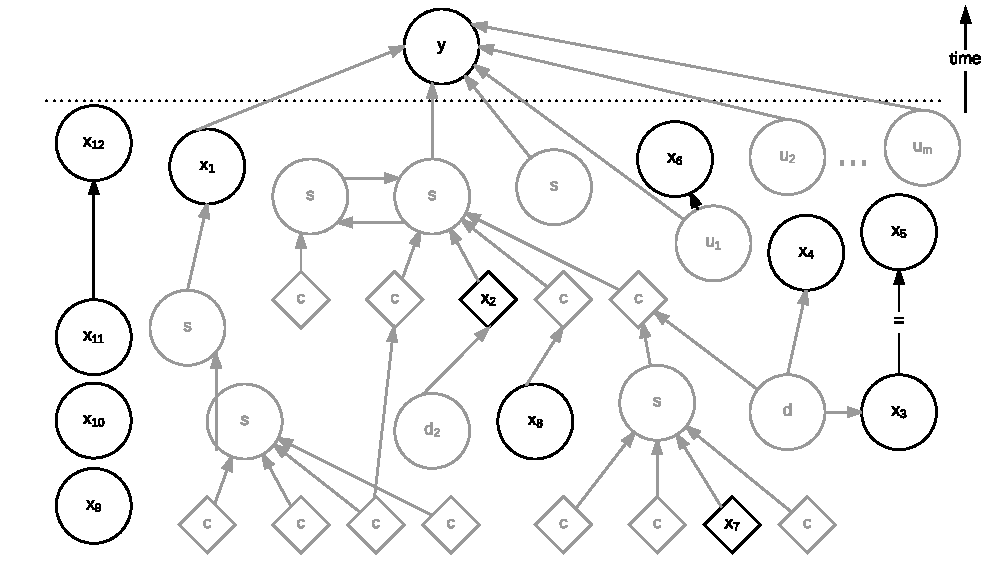
\includegraphics[width=4.1in]{realistic_predictors}
\end{figure}

Grey variables and known to be dependent but the values are unknown and the $u_k$'s are the \qu{unknown unknowns}.

\end{frame}

\begin{frame}\frametitle{Consider Realistic Predictors}

Some observations from the previous illustration:\pause

\begin{itemize}
\item Maybe some of the predictors $x_1, \ldots, x_p$ are causal, but most are likely not. \pause
\item Of the ones that are not causal due to a confounder, you may have an idea of the lurking variables but it is unlikely you can measure them. Think college GPA vs SAT with confounder true IQ / ability.\pause
\item If some variables are causal, it is unlikely they have an additive causal effect; their effect is likely moderated by many other interacting variables possibly in non-linear ways.\pause
\item A linear model for $y$ on $x_1, \ldots, x_p$ is likely far from the truth (not related to our discussion on causality).
\end{itemize}

\end{frame}

\begin{frame}\frametitle{Inference and Causality}

\begin{figure}
\centering
\includegraphics[width=4.5in]{inference_possible}
\end{figure}

\end{frame}

\begin{frame}\frametitle{Sidebar: Theories are Hard...}
\begin{figure}
\centering
\includegraphics[width=3.5in]{theories_are_impossible}
\end{figure}

\footnotesize
Maybe we know the predictors, but don't know the causal dependencies. How many theories are possible? \pause 23 variables, 4 configurations between each pair, 23 possible dependences to the the response ... = \pause $4^{\binom{23}{2}} \times 2^{23} = 1.757 \times 10^{159}$. And that's not even counting the unknown unknowns... thus, many have said that generally speaking \qu{science is \pause impossible} .

\end{frame}

\begin{frame}\frametitle{More on OLS Coefficient Interpretation}

\small
The linear regression coefficient interpretation again: another object \emph{naturally observed} with exactly the same features except that $x_j$ is increased by $1$ unit will have a $\betahat_j \pm \se{\betahat_j}$ difference in its mean response $y$.\\~\\

What do we mean by naturally observed? \pause This other object is realized from the same joint distribution as all other observations. This means that whatever \textit{multicollinearity} / \textit{covariance structure} exists between the predictors, $\braces{\cov{X_j}{X_k}}$, will give rise to the predictor values in the other object.
	
\begin{figure}
\centering
\includegraphics[width=2.8in]{predictor_covariance_structure}
\end{figure}

\end{frame}

\begin{frame}\frametitle{The Hidden \qu{Fifth} OLS Assumption}

So this language \qu{... exactly the same features except that $x_j$ is increased by ...} is \pause kind of absurd in the context of a strong covariance structure as ... \pause i.e. it will be very rare to observe an observation with $x_j$ different without any other predictor values different. Example from baseball dataset? \\~\\ \pause 

There is room to argue that to have these interpretations be at all realistic, we must assume there is not ... \pause  a strong multicollinearity structure between $x_j$ and the other predictors. \pause \\~\\

But isn't getting the adjustments the whole reason we do linear regression??
	
\end{frame}

\begin{frame}\frametitle{But Real Correlations Still Rock}

We've been beating up on correlations and their interpretations e.g. the following:

\begin{figure}
\centering
\includegraphics[width=2.5in]{umbrellas_car_accidents.png}
\end{figure}
\pause

But even though higher umbrella sales do not \qu{cause} accidents, can they still predict them? \pause Yes, $R^2$ is totally agnostic to (a) if your model is true and \pause (b) if your variables are causal or not. Predictors \textit{truly} correlated (a causal link exists) to the response contain information about the value of the response and it doesn't matter through what channel it provides that information. \pause
	
\end{frame}

\begin{frame}\frametitle{Fake / Spurious Correlations}
\pause 
%%from http://io9.gizmodo.com/our-new-favorite-website-spurious-correlations-1574464459

\footnotesize
$x$ is margarine consumption per capita in America measured yearly for 10 years from 2000-2009, $y$ is the divorce rate in Maine per 1000 people measured yearly for 10 years from 2000-2009

\vspace{-0.2cm}
\begin{figure}
\centering
\includegraphics[width=2.2in]{margarine_divorce_time.png}
\end{figure}

\vspace{-0.3cm}
Are they linearly predictive of one another? \pause

\vspace{-0.2cm}
\begin{figure}
\centering
\includegraphics[width=2.2in]{margarine_divorce.png}
\end{figure}
\pause


\vspace{-0.3cm}
$R^2 \approx 99\%$, $F$ test $\pval \approx 1 \times 10^{-8}$. [R demo] 

	
\end{frame}

\section{Mult. Testing}


\begin{frame}\frametitle{Data dredging / mining / p-hacking is a dangerous enterprise}

\small
Be careful about featurization... try to at least have some inkling of an idea for a causal dependency for the response on the predictors... \pause I \qu{found} this using by running that demo code for a few hours...
 
\begin{figure}
\centering
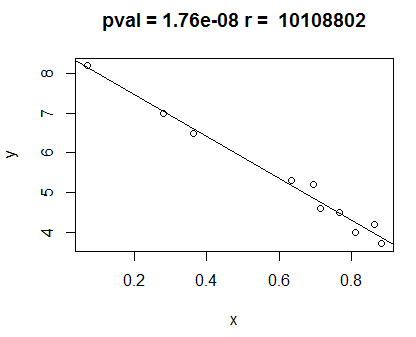
\includegraphics[width=3in]{data_mining.png}
\end{figure}
	
\end{frame}

\begin{frame}\frametitle{Unintential Dredging}
\small
[JMP Baseball data] \pause Consider all these $t$-tests. Is it possible some are true because I've dredged by testing all of them? \pause Of course. \\~\\

\pause When is an individual $t$-test / $F$-test / LR test valid? \pause When you are looking to test one single theory. Imagine you wished to test $H_a: \beta_{\text{num\_RBIs}} \neq 0$. Here's all you \qu{see} then:

\begin{figure}
\centering
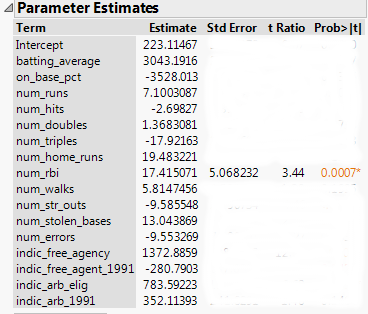
\includegraphics[width=2.1in]{baseball_param_ests.png}
\end{figure}

\end{frame}

\begin{frame}\frametitle{Sidak Correction}
\small
If you \qu{see} all of the parameter tests, what theory were you testing? \pause  Every single one... it is as if you were \qu{looking for \pause  variables} that matter (this is called \emph{variable selection} and we will be doing this later on in the course). But again, that $\alpha := \prob{\text{Type I error}}$ gets you... the false positives. What can we do to curb this? \pause Do a \qu{multiple testing correction}. \\~\\

Imagine $K$ tests. The strictest correction will be when considering that they fail to reject $H_0$ implying that their $p$ values are $\sim \stduniform$. A rejection occurs at $p < \alpha$ which has probability $\alpha$. This is called the false positive rate / Type I error. \\~\\ 


\pause We want to control the \qu{family-wise error rate} (FWER) meaning the probability of one or more Type I errors is $\leq \alpha_{FWER}$.

\footnotesize
\beqn
\alpha_{FWER} &:=& \prob{\geq \text{1 rejection}} = 1 - \prob{\text{0 rejections}} = 1 - \binom{K}{0} \alpha^0 \tothepow{1-\alpha}{K} \\
&=& 1 - (1 - \alpha)^K \eqncomment{AKA the Sidak Correction}
\eeqn

What does this assume among the $K$ tests? \pause Independence.

\end{frame}

\begin{frame}\frametitle{Bonferroni Correction}

\small
What does the Sidak Correction assume among the $K$ tests? \pause Independence. \pause Can we assume that here? \pause No. There is multicollinearity which means $\cov{\betahat_i}{\betahat_j} \neq 0$. What can we do now? Call event $R$ a rejection. Recall inclusion exclusion:

\beqn
\prob{R_1 \cup R_2} &=& \prob{R_1} + \prob{R_2} - \prob{R_1 \cap R_2} \\
\alpha_{FWER} &=& \alpha + \alpha - \fbox{?}
\eeqn

which can be used to demonstrate Boole's Inequality:

\beqn
\prob{\bigcup_{k=1}^K R_k} &\leq& \sum_{k=1}^K \prob{R_k} \\
\alpha_{FWER} &\leq& \sum_{k=1}^K  \alpha = K\alpha
\eeqn

Meaning if I want the typical $\alpha_{FWER} = 5\%$, I'd better set the individual rejection at $5\% / K$. This is known as the Bonferroni Correction.
\end{frame}

\begin{frame}\frametitle{Scheffe Correction}

The Bonferroni Correction is extremely conservative here. Why? \pause Because in OLS, we know the dependence structure. We can somewhat figure out the $\prob{R_1 \cap R_2}$ terms above. One solution from the 1950's is called Scheffe's Method:

\beqn
\prob{\frac{\parens{\bv{\betahat} - \bbeta}^\top \XtXinv \parens{\bv{\betahat} - \bbeta}}{p MSE} \leq F_{\alpha, p, n - p}} = 1 - \alpha
\eeqn

This also account for every possible contrast you'd ever want to test e.g. $H_a: \beta_3 + \beta_7 \neq \beta_5 - \beta_2$. \\~\\ \pause

I can't figure out how to do this in JMP, so if it is on the homework, we will do it in R. 
\end{frame}

\begin{frame}\frametitle{Omnibus $F$ test as a \qu{Correction}}

Recall:

\beqn
R^2 = \frac{SSE_0 - SSE}{SSE_0} = \pause \ldots = 1 - \inverse{1 + F \frac{p-1}{n-p}}
\eeqn

\beqn
F &=& \frac{\frac{SSE_0 - SSE}{p}}{\frac{SSE}{n-p}} \pause  = \frac{SSE_0 - SSE}{SSE} \frac{n-p}{p} = \ldots \\
&=& \underbrace{\frac{R^2}{1-R^2}}_{
%
\substack{
\text{ratio of variance} \\ 
\text{explained to} \\ 
\text{unexplained}
}} 
\times
\underbrace{\frac{n-p}{p}}_{\substack{
\text{penalty for} \\ 
\text{too many features}
}}
\eeqn

[R Demo]

\end{frame}

\section{Equiv. Testing}

\begin{frame}\frametitle{Hypothesis Testing: a Review}

Conceptually, let's act out the introduction of data assuming $H_0$, $H_a$ and some predetermined level $\alpha$. \\~\\

\beqn
&& H_0: \text{UFOs do not exist} \\
&& H_a: \text{UFOs do exist}
\eeqn

and the inverse:

\beqn
&& H_0: \text{UFOs do exist} \\
&& H_a: \text{UFOs do not exist}
\eeqn

\qu{Flipping} the null and the research hypothesis represents a completely different framing. The Type II error is now controlled for.

\end{frame}

\begin{frame}\frametitle{Hypothesis Testing: a Review}

For regression, we can consider the same: \\~\\

\beqn
&& H_0: \beta_j = 0 \\
&& H_a: \beta_j \neq 0
\eeqn

and the inverse:

\beqn
&& H_0: \beta_j \neq 0 \\
&& H_a: \beta_j = 0
\eeqn

[R Demo]

\end{frame}


\begin{frame}\frametitle{An Equivalence Test}

\small
We are trying to prove $\beta_j = 0$ so we first assume $\beta_j \neq 0$ and wait until we have enough evidence (an \qu{equivalence test}). Can you think of a situation you would need this type of control? \\~\\ \pause

We first define $\delta$, a margin of practical equivalence, so if $\beta \in \bracks{-\delta, \delta}$ than practically speaking we believe it to be zero. You need to set $\delta$ yourself. Then we run two tests at level $\alpha$:

\begin{minipage}{0.45\textwidth}

\beqn
&& H_0: \beta_j \geq \delta \\
&& H_a: \beta_j < \delta \\
\eeqn

\end{minipage}
\begin{minipage}{0.45\textwidth}

\beqn
&& H_0: \beta_j \leq -\delta \\
&& H_a: \beta_j > -\delta \\
\eeqn

\end{minipage}

This is known as TOST (two one sided tests) which is equivalent to taking the intersection of two $\alpha$-sized one sided confidence intervals, i.e. a two sided confidence interval at level $2\alpha$. Thus, we reject $H_0$ if:

\beqn
CI_{\beta_j, 1-\alpha} := \bracks{\betahat_j \pm t_{\alpha, n-p-1} \se{\betahat_j}} \in \bracks{-\delta, \delta}
\eeqn

[R demo]


\end{frame}


\section{Design}

\begin{frame}\frametitle{Dataframe Design}

We spoke a lot about featurization i.e. selecting the columns in the dataframe (these are the predictors to measure). Once we did this, we can then go out and sample observations and then measure each for their predictor values. \\~\\ \pause

But we didn't speak at all about selecting the observations themselves (assuming you have some modicum of control of selecting your data). Two things to consider: \\~\\  \pause

\begin{enumerate}
\item \emph{Generalizability} refers to the ability of the model to generalize, or be \emph{externally valid} when considering new observations. This comes down to sampling observations from the same population as your new data you wish to predict (pretty obvious). Sometimes difficult in practice! \pause
\item Optimal Design
\end{enumerate}

	
\end{frame}

\begin{frame}\frametitle{Optimal Design for Inferring one Slope}

Question: assume OLS and that we only care about inference for $\beta_1$. We can sample any $x$ values $\in \bracks{x_m, x_M}$. What should the $n$ values be? \\~\\

Let $x_m = 0$, $x_M = 1$ and $n = 10$. The best inference for $\beta_1$ means ... \pause $\se{\betahat_1}$ is minimum. Design strategies for the $x$'s: \pause

\begin{enumerate}
\item Random sampling \pause
\item Uniform spacing: $\braces{0, 0.111, 0.222, \ldots, 0.999}$ \pause
\item Something else?
\end{enumerate}

[R demo]

\end{frame}


\begin{frame}\frametitle{Optimal Design: Split Between Extremes}

Recall the formula from Stat 102 / 613:

\beqn
\se{\betahat_1} = \sqrt{\frac{MSE}{(n-1)s^2_x}}
\eeqn

How can we make this small?

\begin{enumerate}
\item Maximize $n$ (duh)
\item Minimize the numerator, $MSE$ i.e. minimize the $SSE$. Can we do this? Yes by picking the closest $\betahat_1$ to $\beta_1$ (which we already do). \pause
\item Maximize the denominator $(n-1) s^2_x$. Since $n$ is already maximized, we can pick $x_1, \ldots, x_n$ to maximize $s^2_x$, the sample variance of the predictor.  How? \pause Put half of the $x$'s at $x_m$ and the other half at $x_M$ thereby \pause maximizing the distance from the $x$'s to \pause $\xbar$.
\end{enumerate}
	
\end{frame}

\begin{frame}\frametitle{Optimal Design of Linear Models}
\small

We seek the best linear approximation of $f(x)$ which is $\beta_0 + \beta_1 x _1+ \ldots + \beta_p x_p$. We pick the $\x$'s to give us the best linear approximation. What criteria? JMP gives two ways:

\begin{enumerate}
\item Note: $\var{\betahat_0, \betahat_1, \ldots, \betahat_p} = \sigsq \XtXinv$ \pause

$D$-optimality: maximize $\abss{\XtX}$ --- this maximizes the variance-covariance among the parameter estimates. \pause

\item Note: $\var{\Yhat_1, \ldots, \Yhat_n} = \sigsq \XXtXinvXt$ \pause

$I$-optimality: minimize the average prediction variance over the design space.
\end{enumerate}

[R Demo] \pause What did we learn? \pause For linear models with no polynomials or interactions, keep the observations as close to the minimimums and maximums as possible. For linear models with polynomials and interactions (more non-parametric than parametric), \pause keep most towards the minimums and maximums and some in the center of the input space.

\end{frame}


\section{Extrapolation}


\begin{frame}\frametitle{Extrapolation}
\small
Data driven approaches are all focused on accuracy during \emph{interpolation}.  

\begin{figure}
\centering
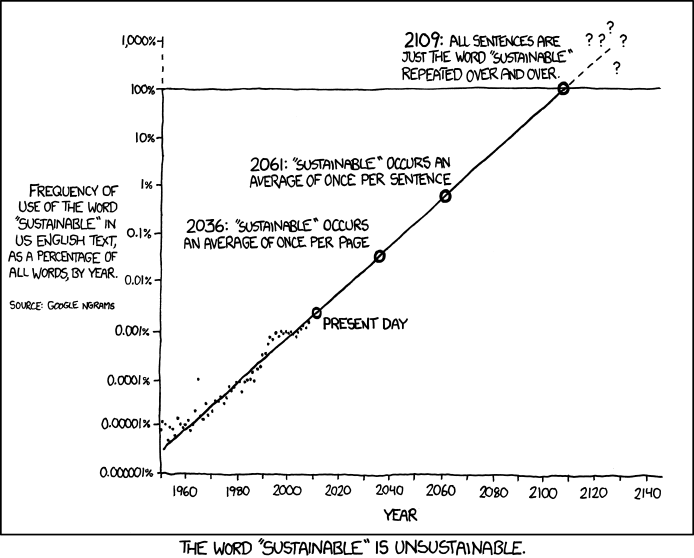
\includegraphics[width=2.5in]{extrap1.png}
\end{figure}
\vspace{-0.3cm}
Extrapolation brings trouble. It is important to ask the question for a new observation $\x^*$ if it is within the space of $\x$'s in the historical data. (Hardly anyone does this... but you should)! Be aware that extrapolation methods of different algorithms differ considerably! [R Demo]
	
\end{frame}

\begin{frame}\frametitle{Reconciliation of those Silly Cartoons}

\begin{figure}
\centering
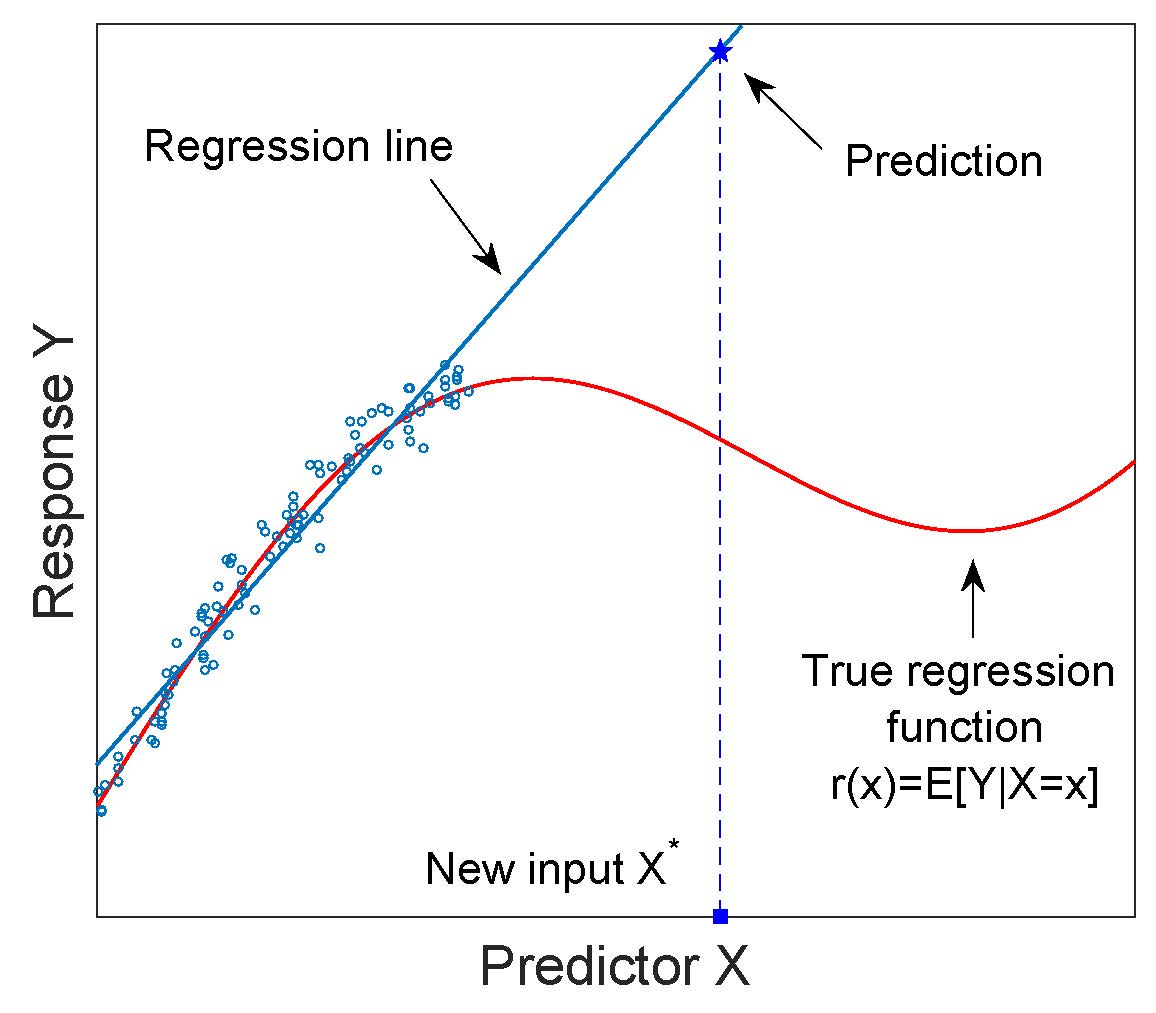
\includegraphics[width=3.2in]{extrap.jpg}
\end{figure}

\end{frame}

\section{Logistic Regression}


\begin{frame}\frametitle{Modeling Categorical Responses}

Previously the response $y$ was continuous and via the OLS assumptions we obtained the statistical model,

\beqn
Y \inddist \normnot{\beta_0 + \beta_1 x_1 + \ldots + \beta_p x_p}{\sigsq}
\eeqn

If the response $y$ is categorical, can we still use this? \pause No... the only elements in the support of the r.v. $Y$ are the levels only. [JMP Churn] \\~\\

First, assume $Y$ is binary i.e. zero or one. The model we use is...\pause  

\beqn
Y \sim \bernoulli{f(x_1, \ldots, x_p)}
\eeqn

since $\cexpe{Y}{x_1, \ldots, x_p} = f(x_1, \ldots, x_p)$, then $f$ is still the conditional expectation function like before except now it varies only within \pause $\zeroonecl$ and it is the same as \pause   $\cprob{Y = 1}{x_1, \ldots, x_p}$.

\end{frame}

\begin{frame}\frametitle{Linear $f(x)$?}

We can model $f(x)$ as the simple linear function but this returns values smaller than 0 and larger than 1 and thus it cannot be the conditional expectation function! Why? \pause Lines vary between $\parens{-\infty, +\infty}$. \\~\\ \pause

We need a \qu{link function} to connect the linear function to the restricted support of the response:

\beqn
\lambda(f_{\reals}(x_1, \ldots, x_p)) = f(x_1, \ldots, x_p)
\eeqn

And the parametric assumption would be

\beqn
\lambda(s_{\reals}(x_1, \ldots, x_p; \theta_1, \ldots, \theta_\ell)) = s(x_1, \ldots, x_p; \theta_1, \ldots, \theta_\ell)
\eeqn

And assuming a linear form:

\beqn
\lambda(\beta_0 + \beta_1 x_1 + \ldots + \beta_p x_p) = ?
\eeqn

\end{frame}

\begin{frame}\frametitle{Choice of $\lambda$?}

We just need $\lambda: \reals \rightarrow \zeroonecl$. There are infinite $\lambda$'s to choose from. I've only seen three used: \pause

\begin{enumerate}
\item Logistic link: $\lambda(w) = \frac{e^w}{1 + e^w}$ (most common) \pause
\item Inverse normal (probit) link: $\lambda(w) = \Phi^{-1}(w)$ where $\Phi$ is the normal CDF function (somewhat common) \pause
\item Complementary Log-log (cloglog) link: $\lambda(w) = \natlog{-\natlog{w}}$ (rare!)
\end{enumerate}

Let's investigate what the first one means. Define $p := \prob{Y=1}$. We can think about probability  in another way:

\beqn
odds(Y = 1) := \frac{p}{1-p}
\eeqn

So if odds = 4:1, what is $p$? This means that the probability of the event happening is four times more likely than the complement happening. Or...  of 4+1 runs, 4 will be a yes. What is the range of odds? \pause $[0, \infty)$.
	
\end{frame}

\begin{frame}\frametitle{Why Logistic Link is Interpretable}
\small
Now let's take the log odds (called the logit function):

\beqn
logit(Y = 1) := \natlog{odds(Y = 1)} = \natlog{\frac{p}{1-p}}
\eeqn

What is the range of the logit function? \pause All of $\reals$. Hence, we can now set this equal to our \pause $s_\reals$ function. In the linear modeling context,

\footnotesize
\beqn
\beta_0 + \beta_1 x_1 + \ldots + \beta_p x_p &=& logit(Y = 1) =  \natlog{\frac{p}{1-p}} \\ \pause
e^{\beta_0 + \beta_1 x_1 + \ldots + \beta_p x_p} &=& \frac{p}{1-p} \\ \pause
(1-p)e^{\beta_0 + \beta_1 x_1 + \ldots + \beta_p x_p} &=& p \\ \pause
e^{\beta_0 + \beta_1 x_1 + \ldots + \beta_p x_p}  &=& p + p e^{\beta_0 + \beta_1 x_1 + \ldots + \beta_p x_p}\\ \pause
p &=& \frac{e^{\beta_0 + \beta_1 x_1 + \ldots + \beta_p x_p}}{1 + e^{\beta_0 + \beta_1 x_1 + \ldots + \beta_p x_p}} = \lambda(\beta_0 + \beta_1 x_1 + \ldots + \beta_p x_p) \pause
\eeqn

\small
Thus, a change in the linear model becomes a linear change in log-odds. This is (I would say) the most interpretable link function situation we've got.
	
\end{frame}

\begin{frame}\frametitle{The Logistic Function}

\begin{figure}
\centering
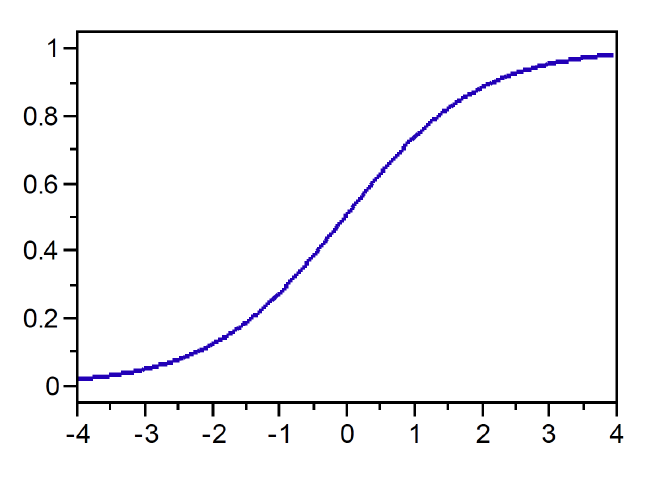
\includegraphics[width=3.2in]{logistic_function.png}
\end{figure}

\end{frame}

\begin{frame}\frametitle{How to Obtain a Model Fit}

A model fit would mean we estimate $\braces{\betahat_0, \betahat_1,  \ldots, \betahat_p}$. We initially did this estimation for regression (continuous $y$) by defining a loss function, SSE, and finding the optimal solution via calculus. What do we do now?? \\~\\

Likelihood to the rescue. First the \qu{logistic regression assumptions}

\begin{enumerate}
\item Linear-Logistic conditional expectation \pause
\item Independence
\end{enumerate}

\small
\beqn
&&\cprob{Y_1 = y_1, Y_2 = y_2, \ldots, Y_n = y_n}{\X_1 = \x_1, \X_2 = \x_2, \ldots, \X_n = \x_n} \\
&=& \prod_{i=1}^n \cprob{Y_i = y_i}{\X_1 = \x_i}
\eeqn

How?
	
\end{frame}

\begin{frame}\frametitle{Maximum Likelihood Estimates}
\small
\beqn
= \prod_{i=1}^n p^{y_i} (1-p)^{1-y_i}
\eeqn

How? \pause

\beqn
= \prod_{i=1}^n \parens{\frac{e^{\beta_0 + \beta_1 x_1 + \ldots + \beta_p x_p}}{1 + e^{\beta_0 + \beta_1 x_1 + \ldots + \beta_p x_p}}}^{y_i} \parens{1 - \frac{e^{\beta_0 + \beta_1 x_1 + \ldots + \beta_p x_p}}{1 + e^{\beta_0 + \beta_1 x_1 + \ldots + \beta_p x_p}}}^{1-y_i}
\eeqn

How? \pause This does not have a simple, closed form solution. The computer iterates numerically and converges on the values of the parameters that maximize the above and these are shipped to you as $\braces{\betahat_0, \betahat_1,  \ldots, \betahat_p}$. This is called \qu{running a logistic regression}.
	
\end{frame}

\begin{frame}\frametitle{Prediction with Logistic Regression}

How? \pause

\beqn
\phat = \phat(x^*_1, \ldots, x^*_p) = \pause \frac{e^{\betahat_0 + \betahat_1 x_1 + \ldots + \betahat_p x_p}}{1 + e^{\betahat_0 + \betahat_1 x_1 + \ldots + \betahat_p x_p}}
\eeqn
	
\end{frame}


\end{document}
	


\begin{frame}\frametitle{}

	
\end{frame}

\begin{frame}\frametitle{}

	
\end{frame}

\begin{frame}\frametitle{}

	
\end{frame}






\begin{frame}\frametitle{}

	
\end{frame}



\begin{frame}\frametitle{}

	
\end{frame}

\begin{frame}\frametitle{}

	
\end{frame}


\begin{frame}\frametitle{}

	
\end{frame}

\begin{frame}\frametitle{}

	
\end{frame}


\begin{frame}\frametitle{}

	
\end{frame}

\begin{frame}\frametitle{}

	
\end{frame}


\begin{frame}\frametitle{}

	
\end{frame}

\begin{frame}\frametitle{}

	
\end{frame}


\begin{frame}\frametitle{}

	
\end{frame}

\begin{frame}\frametitle{}

	
\end{frame}


\begin{frame}\frametitle{}

	
\end{frame}

\begin{frame}\frametitle{}

	
\end{frame}


\begin{frame}\frametitle{}

	
\end{frame}

\begin{frame}\frametitle{}

	
\end{frame}


\begin{frame}\frametitle{}

	
\end{frame}

\begin{frame}\frametitle{}

	
\end{frame}


\begin{frame}\frametitle{}

	
\end{frame}

\begin{frame}\frametitle{}

	
\end{frame}